\documentclass[runningheads]{llncs}

\usepackage[T1]{fontenc}
\usepackage{graphicx}
\usepackage{booktabs}
\usepackage{amsmath}
\usepackage{amssymb}
\usepackage{float}
\usepackage{url}
\usepackage{rotating}

\begin{document}

\title{Bridging Text and Graph Topology for Wikipedia Article Recommendation}
\titlerunning{Text and Graph Topology for Recommendation}

\author{Sahin Uregil\inst{1}\thanks{Corresponding author: uregilsahin@gmail.com} \and G\"unce Keziban Orman\inst{1}}
\authorrunning{S. Uregil and G. K. Orman}

\institute{Department of Computer Engineering, Galatasaray University, Istanbul, T\"urkiye\\
\email{uregilsahin@gmail.com, korman@gsu.edu.tr}}

\maketitle

\begin{abstract}
Article recommendation systems identify relevant articles based on reader preferences and reading history. Existing approaches include collaborative filtering, matrix factorization, content-based methods, and neural network-based models. Recently, Graph Neural Networks (GNNs) have become central to article recommendation by leveraging article network structure. These systems are often evaluated on benchmarks such as Cora, CiteSeer, PubMed, and Wiki-CS. Among them, Wiki-CS is widely used due to its open-source accessibility, graph-ready structure, and representation of Wikipedia articles as nodes with directed hyperlink edges. Article text can also be embedded and used as node attributes, enabling richer representations.

This study presents a graph-based article-to-article recommendation framework centered on hybrid semantic-structural retrieval. We combine sentence embeddings with structural representations from Node2Vec, and study corrected Node2Vec variants together with hybrid models that fuse text and graph structure. We also investigate pooled semantic representations designed to balance textual and structural signals, yielding corrected hybrid models with the most balanced recommendation quality in our experiments. We benchmark semantic, structural, hybrid, and GNN-based models under a revised evaluation protocol, showing that carefully designed hybrid retrieval is more reliable than single-source baselines.

To support this setting, we introduce a reconstructed and up-to-date version of Wiki-CS. The reconstruction resolves the lack of usable raw text in the original benchmark by cleaning and aligning article titles, recovering article text through integration with the Wikipedia STEM corpus and Wikipedia API, and applying state-of-the-art embedding models to the reconstructed collection. This provides complete raw text for every active node and enables reproducible, up-to-date recommendation experiments with modern Transformer-based text representations.

\keywords{Article recommendation \and Graph recommendation \and Hybrid retrieval \and Wikipedia graphs \and Benchmark reconstruction}
\end{abstract}

\section{Introduction}

Article recommendation can be studied under several settings. Many widely used
systems rely on user behavior, collaborative signals, or historical interaction
patterns. The setting considered in this paper is different: given a source
Wikipedia article, the objective is to retrieve a ranked list of related
articles that are both semantically relevant and structurally meaningful in the
 hyperlink graph. This article-to-article formulation is useful when explicit
user histories are unavailable, when interpretability matters, or when the goal
is guided exploration of a knowledge domain rather than personalized
consumption.

Wikipedia is a natural graph environment for this task. Its hyperlink structure
encodes editorial and conceptual relations, while article text provides a dense
semantic signal that can reveal topical proximity even when direct links are
missing. These two sources of information are complementary, but they are not
always easy to combine in a way that preserves both topological context and
textual meaning. This makes Wikipedia article recommendation a suitable testbed
for hybrid semantic-structural retrieval.

The starting point of this work is Wiki-CS, a widely used benchmark derived
from Wikipedia and originally designed for node classification
experiments~\cite{mernyei2020wikics}. Although Wiki-CS offers a graph-ready
representation and broad accessibility, it does not directly provide a
text-complete, up-to-date benchmark for article recommendation with modern text
encoders. This creates two related needs: an updated dataset layer with
recoverable article text, and a recommendation framework able to compare
semantic, structural, hybrid, and GNN-based approaches under a shared
evaluation setting.

This paper addresses both needs. First, we reconstruct Wiki-CS into a
text-enriched benchmark, Custom-WikiCS, by aligning titles, recovering article
text, and attaching modern embedding representations. Second, we introduce a
graph-based article recommendation framework built around semantic retrieval,
Node2Vec-based structural retrieval, corrected structural variants, pooled
semantic-structural hybrids, and graph-neural baselines. Third, we evaluate
these model families under a revised undirected protocol that is better aligned
with the structural view of the task.

The main contributions of the paper are:
\begin{itemize}
\item a reconstructed version of Wiki-CS, denoted Custom-WikiCS, with complete
      raw text for every active node and support for modern text embedding
      pipelines;
\item a hybrid recommendation framework that combines sentence embeddings with
      Node2Vec-derived structural signals, including corrected structural
      variants and pooled semantic fusion;
\item a comparative benchmark across semantic, structural, hybrid, and GNN
      baselines under a revised evaluation protocol for article-to-article
      recommendation.
\end{itemize}

\section{Related Work}

Wikipedia can be modeled naturally as a graph whose nodes are articles and
whose edges are hyperlinks. This makes it a practical environment for graph
representation learning and graph-based recommendation. Wiki-CS provides one of
the most widely reused Wikipedia-derived graph benchmarks in graph learning
research~\cite{mernyei2020wikics}, although its original use case is node
classification rather than article recommendation. More directly related work
includes WikiRecNet, which studies large-scale Wikipedia recommendation using
graph structure and representation learning~\cite{wikirecnet2020}. One lesson
from this line of work is that structural proximity is informative, but
recommendation quality should not be reduced to a generic graph prediction task.

Textual embeddings provide a second major signal family. Transformer-based
encoders~\cite{vaswani2017attention} and BERT-style models~\cite{devlin2019bert}
have made dense semantic retrieval practical at sentence and document level.
Sentence-BERT~\cite{reimers2019sentencebert} further showed how BERT-like
architectures can be adapted for efficient similarity search. More recent
retrieval-oriented models, such as BGE-M3~\cite{chen2025bgem3}, are explicitly
designed for strong dense retrieval across multilingual settings and thus fit
the recommendation scenario considered here.

Structural embeddings capture graph position, local neighborhood, and community
patterns directly from the edge structure. Node2Vec~\cite{grover2016node2vec}
is one of the most influential methods in this family, learning node
representations from random-walk contexts. In recommendation settings,
structural embeddings can recover relations that text alone may miss, although
they can also become sensitive to hub effects and graph-specific artifacts if
the evaluation protocol is not carefully aligned with the structural task.

Graph neural networks provide another structural modeling family. GCN remains a
standard transductive baseline~\cite{kipf2017semi}, while
GraphSAGE~\cite{hamilton2017inductive} introduces neighborhood aggregation with
an inductive flavor. Survey work on GNNs for text-related settings suggests
that these models remain central at the interface of graph structure and
linguistic representation~\cite{li2022graph}. In parallel, multimodal and
hybrid recommender systems increasingly combine text and graph signals rather
than relying on either source alone~\cite{zhou2023multimodal}. Practical hybrid
examples based on BERT and GNN components also show that fusion design can
change retrieval behavior substantially~\cite{anime_hybrid_gnn_bert}.

The present work is positioned at the intersection of these directions. It uses
Wikipedia as a graph recommendation environment, updates a widely used benchmark
to support modern text modeling, and compares semantic, structural, hybrid, and
GNN-based article recommendation models within one experimental framework.


\section{Method}
\subsection{Custom-WikiCS Reconstruction}

\subsubsection{Motivation and Reconstruction Pipeline}

The original Wiki-CS graph is useful as a structural benchmark, but it is less
convenient for modern article recommendation because the benchmark is graph-ready
without being text-complete for current retrieval pipelines. In particular, the
node set is easy to load as a graph, yet the benchmark does not directly expose
the reconstructed raw article text needed to regenerate semantic features with
modern encoders. For a recommendation setting centered on article-to-article
retrieval, this is a practical limitation: text quality and text availability are
not auxiliary metadata, but part of the representation being evaluated.

Custom-WikiCS addresses this limitation through a reconstruction pipeline with
three main stages. First, article titles are cleaned and aligned in order to
improve consistency across graph records, the Wikipedia STEM corpus\footnote{\url{https://www.kaggle.com/datasets/conjuring92/wiki-stem-corpus}}, and API
lookups. This stage resolves naming mismatches, formatting inconsistencies, and
stale title variants that would otherwise prevent article recovery. Second, raw
article text is recovered by combining the Wikipedia STEM corpus with Wikipedia
API backfilling, producing a text-complete collection for the active article
set. Third, the reconstructed collection is used to generate modern text
representations, enabling semantic retrieval models and hybrid recommendation
variants on top of the same graph. In the final reconstructed benchmark, every
active node is associated with usable article text and can therefore participate
in both structural and semantic evaluation.

After reconstruction and cleaning, isolated nodes are removed and the final
graph contains the statistics reported in Table~\ref{tab:dataset-stats}. The
resulting benchmark supports both graph-structural experiments and modern
text-based retrieval on the same article set.

\begin{table}[H]
\caption{Custom-WikiCS graph statistics after reconstruction and cleaning}
\label{tab:dataset-stats}
\centering
\begin{tabular}{lr}
\toprule
\textbf{Statistic} & \textbf{Value} \\
\midrule
Initial nodes & 11,701 \\
Removed isolates & 334 \\
Active nodes & 11,367 \\
Directed edges & 291,039 \\
Undirected edges & 216,123 \\
\bottomrule
\end{tabular}
\end{table}

\subsubsection{Graph Characteristics}

The cleaned graph exhibits a heavy-tailed degree distribution, indicating that a
small number of hub articles coexist with a much larger set of lower-degree
nodes. This matters for article recommendation because purely structural methods
can become dominated by hubs if degree effects are left untreated. The degree
statistics are also strongly skewed in the cleaned graph: total degree ranges
from 1 to 3,474, with mean 51.21 and median 16. This gap between mean and median
is consistent with a hub-dominated article network rather than a uniformly mixed
graph. The left panel of Fig.~\ref{fig:dataset-struct-sem} visualizes the same
behavior on log-log axes and supports the power-law-style correction heuristic
introduced later in the recommendation framework.

At the same time, the graph is semantically assortative. Linked article pairs
are substantially closer in the semantic embedding space than randomly sampled
pairs: under cosine similarity, the linked mean is 0.5726 while the random mean
is 0.4352. This is important because it shows that hyperlink connectivity and
textual meaning are aligned rather than independent. In other words, semantic
retrieval is not being imposed on an unrelated graph; it operates on a benchmark
where the link structure already carries topic-level coherence. The right panel
of Fig.~\ref{fig:dataset-struct-sem} summarizes this effect.

\begin{figure}[t]
\centering
\begin{minipage}[t]{0.47\textwidth}
\centering
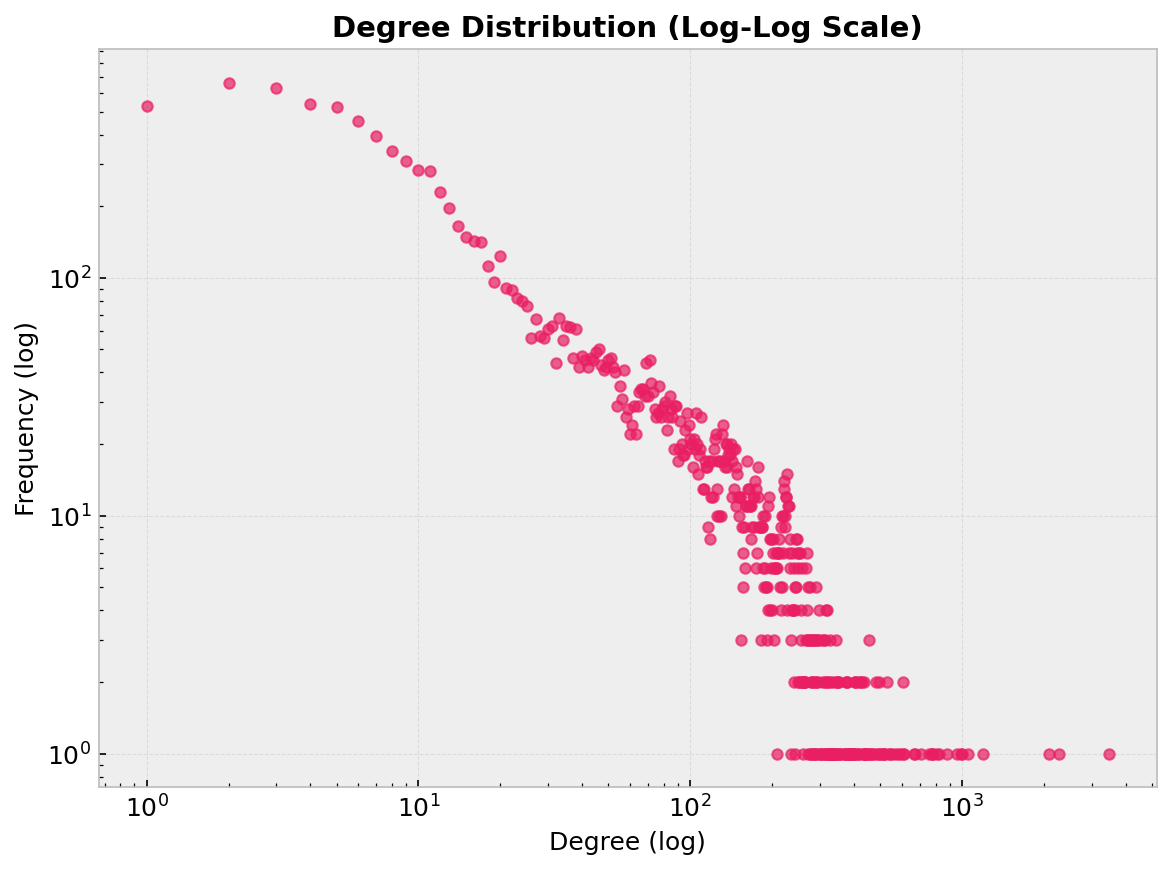
\includegraphics[width=\textwidth]{figs/degree-log-log.png}
\par\small (a) Log-log degree distribution
\end{minipage}\hfill
\begin{minipage}[t]{0.49\textwidth}
\centering
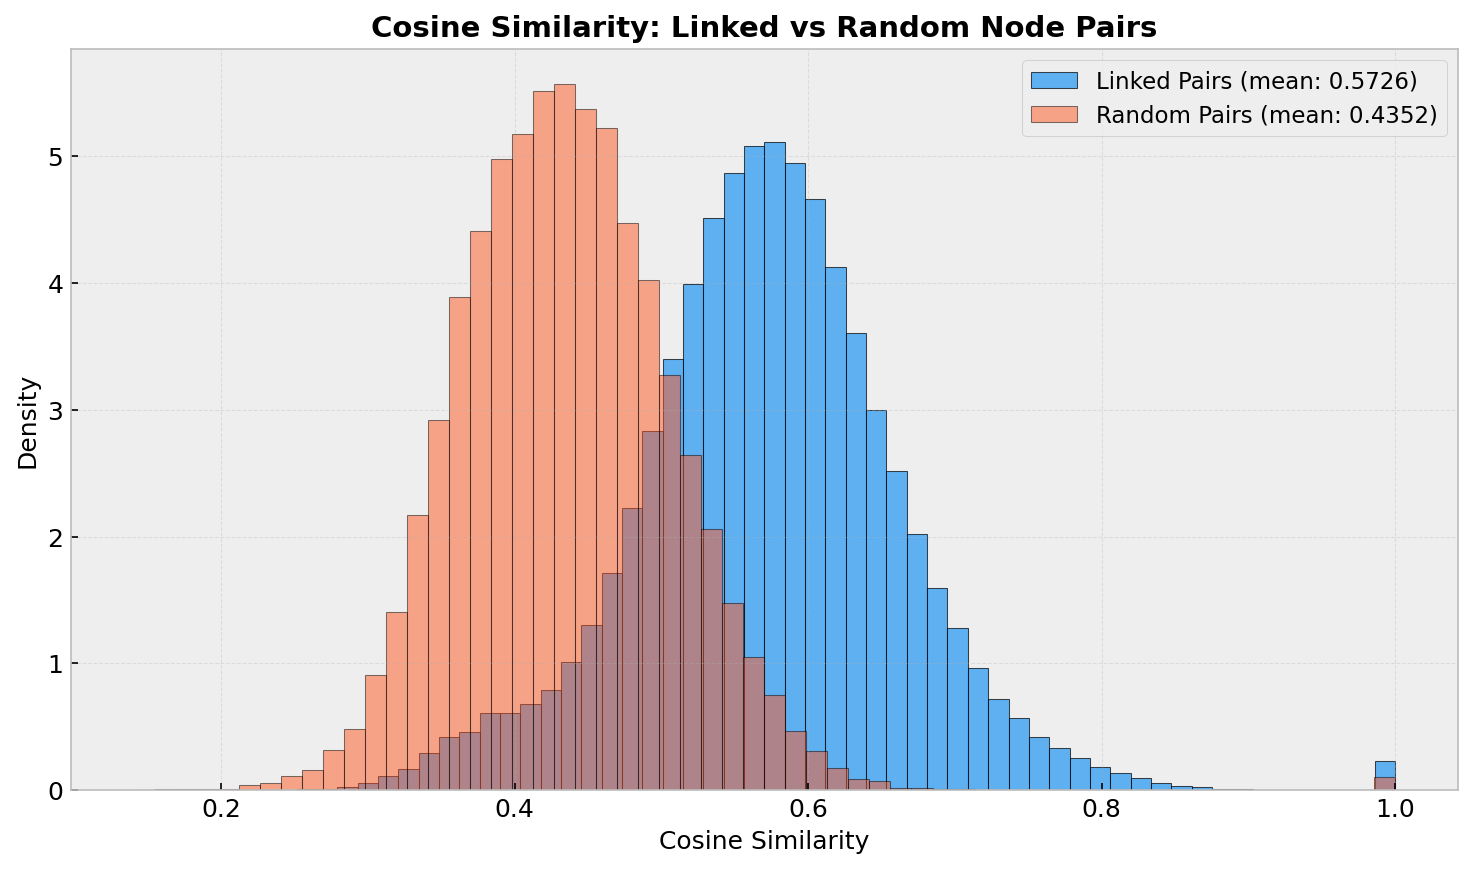
\includegraphics[width=\textwidth]{figs/cosine-similarity-assortativity.png}
\par\small (b) Linked vs.\ random cosine similarity
\end{minipage}
\caption{Structural and semantic diagnostics of Custom-WikiCS. The degree profile is heavy-tailed, while linked article pairs are semantically closer than random pairs in the BGE-M3 embedding space}
\label{fig:dataset-struct-sem}
\end{figure}

Community analysis further shows that the graph is neither flat nor uniformly
mixed. Louvain detection yields modularity
0.6476 over 38 communities, with a largest community of 2,040 nodes and mean
community size 299.13. This confirms that the cleaned graph contains broad topic
regions rather than a single homogeneous article pool. Moreover, the semantic
coherence of these communities is measurable: intra-community cosine similarity
is higher than inter-community similarity under both Louvain (0.5729 vs.\ 0.5435)
and Infomap (0.5748 vs.\ 0.5480). This means that graph communities are not only
topological partitions but also semantically coherent article groupings. Such a
structure is useful for recommendation because it creates meaningful local
neighborhoods beyond direct edge presence. Figure~\ref{fig:community-diagnostics}
summarizes the community-size distribution together with the intra/inter
community similarity comparison.

\begin{figure}[t]
\centering
\begin{minipage}[t]{0.41\textwidth}
\centering
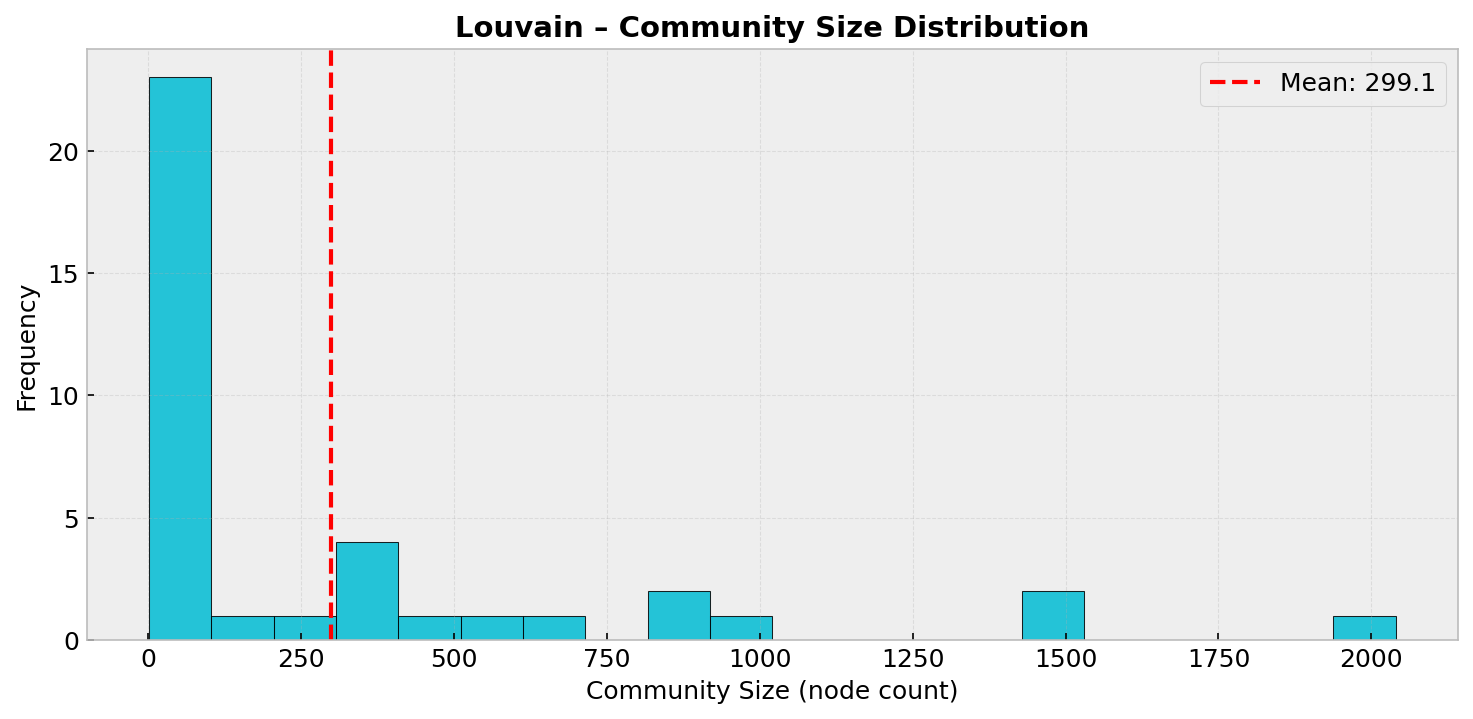
\includegraphics[width=\textwidth]{figs/community-size-distribution-louvain.png}
\par\small (a) Louvain community size distribution
\end{minipage}\hfill
\begin{minipage}[t]{0.55\textwidth}
\centering
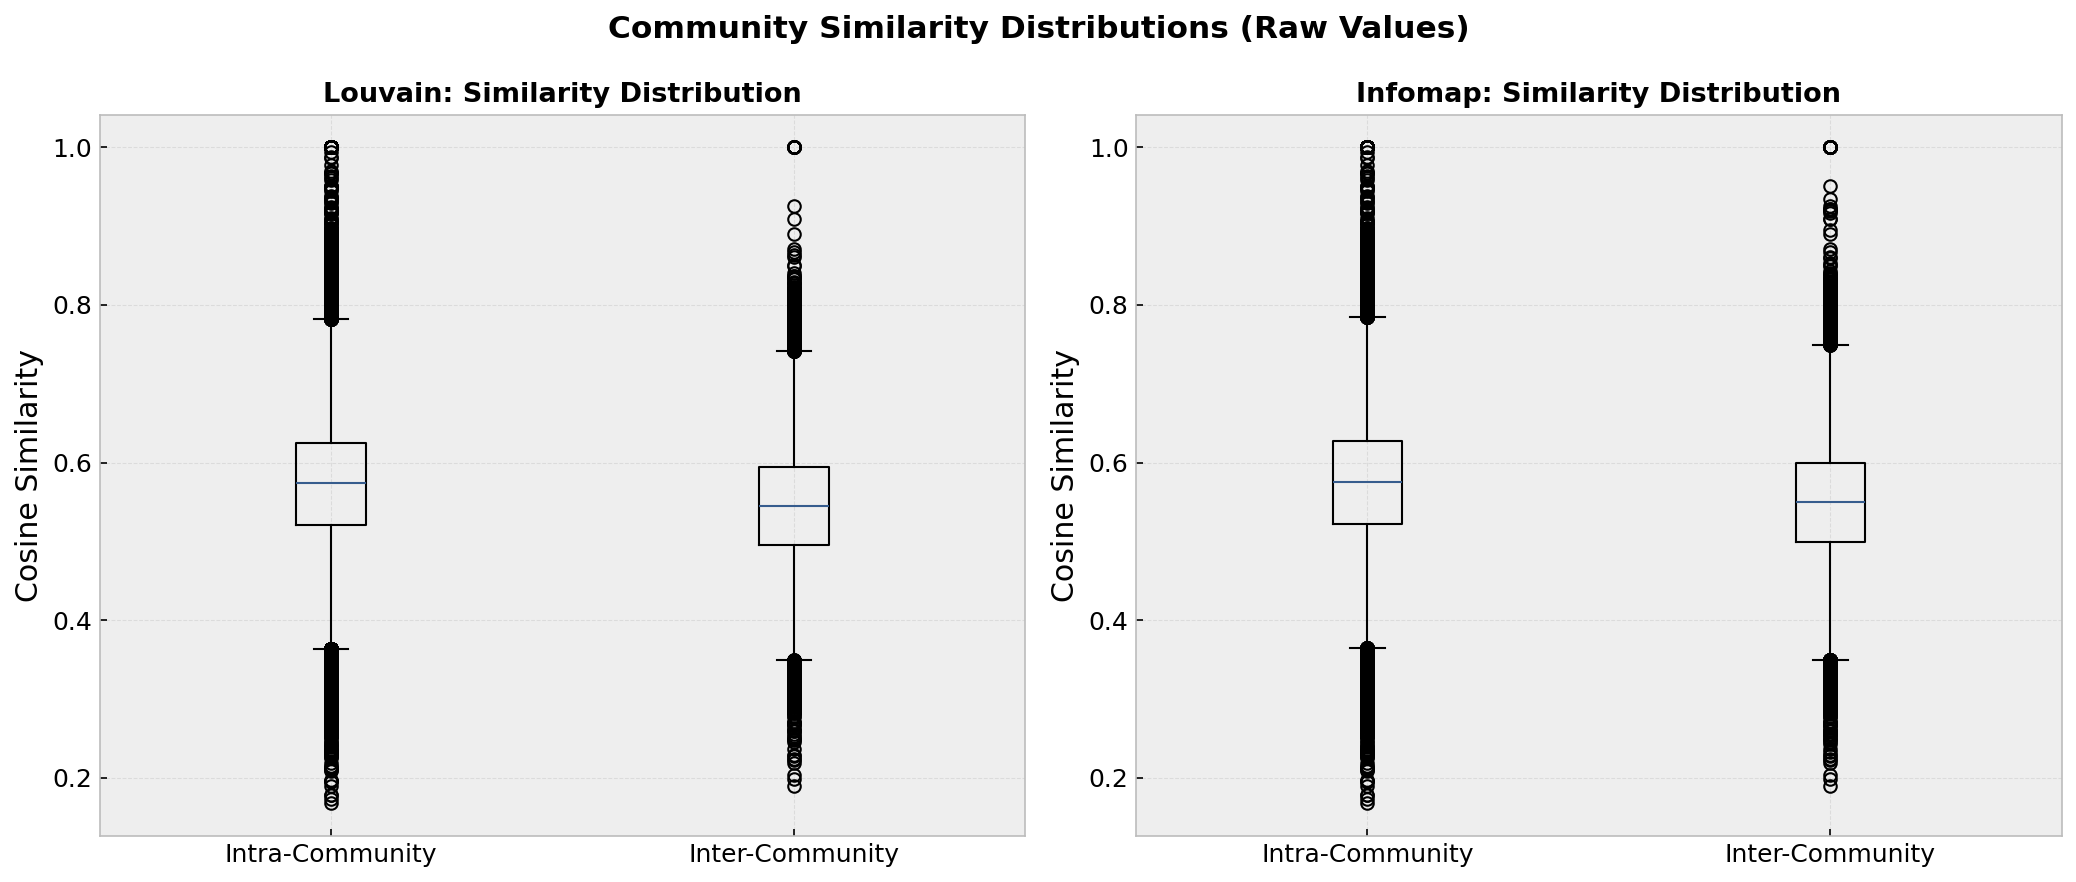
\includegraphics[width=\textwidth]{figs/similarity-distributions.png}
\par\small (b) Intra- vs.\ inter-community similarity
\end{minipage}
\caption{Community diagnostics for Custom-WikiCS. The cleaned graph contains non-trivial communities, and those communities remain semantically coherent}
\label{fig:community-diagnostics}
\end{figure}

\subsection{Recommendation Framework}

\subsubsection{Task Definition}

Let $G=(V,E)$ denote the reconstructed article graph. For a source article
$u\in V$, the goal is to return a ranked list of candidate articles
$v\in V\setminus\{u\}$ that are relevant to $u$ under semantic, structural, or
hybrid similarity. The task is query-based and article-centric: the source
article serves as the query, and the recommendation model ranks all remaining
articles accordingly.

\begin{figure}[H]
\centering
\setlength{\fboxsep}{6pt}
\resizebox{0.78\textwidth}{!}{
\begin{tabular}{c c}
\fbox{\parbox{0.27\textwidth}{\centering Cleaned article titles\\and recovered raw text}} &
\fbox{\parbox{0.27\textwidth}{\centering Cleaned hyperlink\\graph}} \\[0.6em]
$\downarrow$ & $\downarrow$ \\[0.4em]
\fbox{\parbox{0.27\textwidth}{\centering BGE-M3 semantic\\embeddings}} &
\fbox{\parbox{0.27\textwidth}{\centering Node2Vec structural\\embeddings}} \\[0.4em]
\multicolumn{2}{c}{$\searrow \hspace{7em} \swarrow$} \\[0.2em]
\multicolumn{2}{c}{\fbox{\parbox{0.48\textwidth}{\centering Hybrid retrieval model\\(full or pooled semantic signal + optional degree-corrected structural signal)}}} \\[0.4em]
\multicolumn{2}{c}{$\downarrow$} \\[0.2em]
\multicolumn{2}{c}{\fbox{\parbox{0.42\textwidth}{\centering Normalization and cosine ranking over candidate articles}}}
\end{tabular}
}
\caption{Flagship hybrid recommendation pipeline used in the paper}
\label{fig:paper-pipeline}
\end{figure}

\subsubsection{Semantic Retrieval}

The semantic component uses BGE-M3 text embeddings~\cite{chen2025bgem3}. Each
article is represented by a 1024-dimensional dense vector derived from its
reconstructed text. Recommendation scores in the semantic-only setting are
computed by cosine similarity between source and candidate embeddings:
\begin{equation}
s_{\mathrm{sem}}(u,v)=\cos(\mathbf{b}_u,\mathbf{b}_v).
\end{equation}

This component captures semantic proximity even when the hyperlink relation is
sparse or absent, and it serves as both a standalone baseline and one component
of the hybrid models.

\subsubsection{Structural Retrieval}

The structural component uses Node2Vec-style representations~\cite{grover2016node2vec}
computed on the Wikipedia hyperlink graph. Two structural variants are
considered. The first is an uncorrected Node2Vec configuration, which ranks candidates
using cosine similarity in the structural embedding space:
\begin{equation}
s_{\mathrm{str}}(u,v)=\cos(\mathbf{n}_u,\mathbf{n}_v).
\end{equation}
The second is a corrected variant that applies a power-law degree penalty during structural
scoring in order to reduce the tendency of high-degree hubs to dominate
retrieval.

Following the project reports, the correction factor for a node $v$ with
undirected degree $d_v$ is defined as
\begin{equation}
p_v = \log(d_v + 1)^{\alpha},
\end{equation}
where the exponent is estimated from the structural training graph and is
approximately $\alpha \approx 2.9966$ in the revised evaluation setting. The
logarithm softens the extreme upper tail of the degree distribution, while the
power exponent preserves a stronger penalty for structurally over-connected
nodes. The
corrected structural score becomes
\begin{equation}
s_{\mathrm{corr}}(u,v)=\frac{\cos(\mathbf{n}_u,\mathbf{n}_v)}{p_u p_v}.
\end{equation}

\subsubsection{Hybrid and GNN-Based Models}

The central model family of this paper combines semantic and structural
representations. We evaluate four main hybrid variants:
\begin{itemize}
\item direct concatenation of BGE-M3 and uncorrected Node2Vec;
\item direct concatenation of BGE-M3 and corrected Node2Vec;
\item pooled BGE-M3 with uncorrected Node2Vec;
\item pooled BGE-M3 with corrected Node2Vec.
\end{itemize}

In the pooled variants, the 1024-dimensional semantic representation is reduced
to 128 dimensions by block-wise pooling before concatenation, making the
semantic and structural components more comparable in scale. This produces a
256-dimensional hybrid representation rather than the 1152-dimensional vector
obtained by direct concatenation.

More explicitly, the non-pooled hybrid representation is formed as
\begin{equation}
\mathbf{h}_u = [\mathbf{b}_u ; \mathbf{n}_u],
\end{equation}
while the pooled representation uses a reduced semantic vector
$\bar{\mathbf{b}}_u \in \mathbb{R}^{128}$ obtained from contiguous blocks of the
original BGE-M3 embedding:
\begin{equation}
\mathbf{h}^{\mathrm{pool}}_u = [\bar{\mathbf{b}}_u ; \mathbf{n}_u].
\end{equation}
In corrected hybrids, the same degree-normalized structural signal is used
before concatenation. After construction, the hybrid vectors are normalized and
ranked by cosine similarity against all candidate articles. The purpose of
pooling is not to create a new semantic encoder, but to prevent the 1024-dimensional
text representation from numerically overwhelming the 128-dimensional
structural contribution.

The benchmark also includes GCN and GraphSAGE structural baselines, as well as
a ranking-level fusion baseline combining GCN and BGE-M3. Together, these
models span semantic-only, structural-only, hybrid-concatenative, rank-fusion,
and GNN-based retrieval families.

\section{Experiments and Results}

%\subsection{Evaluation Protocol}

All main results reported in this paper use the revised undirected structural
evaluation protocol. Starting from the undirected version of the cleaned graph,
we construct a split with 216,123 undirected edges, of which 172,900 are used
for training and 43,223 for testing. To align ranking evaluation with
article-to-article retrieval, each undirected test edge $\{u,v\}$ is expanded
into two directed queries, $u\rightarrow v$ and $v\rightarrow u$, yielding
86,446 evaluation pairs over 9,022 evaluation nodes.

This revised protocol plays an important methodological role. Earlier project
stages also reported results on held-out directed edges, but the later
comparison in this paper is intentionally centered on the undirected structural
graph because Node2Vec neighborhoods, community analysis, and the degree
correction heuristic are all defined over that structural view. The revised
protocol therefore preserves the article-to-article ranking task while aligning
the training structure, the correction heuristic, and the evaluation target more
closely than a purely directed holdout would.

The experimental workflow is notebook-centered and relies on cached structural
and semantic artifacts generated from the reconstructed dataset. The benchmark
includes semantic, structural, hybrid, and GNN-based models evaluated under the
same underlying revised split, making the reported comparisons directly
comparable at the level of ranking outputs.

\subsection{Evaluation Metrics}

Let \(Q\) denote the set of evaluation queries, let \(r_q\) be the rank of the
held-out target article for query \(q\), and let \(L_q\) be the returned
recommendation list. Our ranking metrics follow standard information retrieval
practice~\cite{manning2008ir,voorhees1999trec8qa}. Because each query has
exactly one held-out target in the ranking protocol, several metrics simplify.
The basic top-list metrics are

\begin{equation}
\text{Hit@}K = \frac{1}{|Q|}\sum_{q \in Q} \mathbf{1}[r_q \le K]
\end{equation}



\begin{equation}
\text{MRR} = \frac{1}{|Q|}\sum_{q \in Q} \frac{1}{r_q}
\end{equation}
For the same single-target setting, normalized discounted cumulative gain
reduces to
\begin{equation}
\text{NDCG@}K = \frac{1}{|Q|}\sum_{q \in Q}
\frac{\mathbf{1}[r_q \le K]}{\log_2(r_q + 1)}
\end{equation}
since the ideal DCG of one relevant item equals \(1\). Likewise,
\begin{equation}
\text{Recall@}K = \text{Hit@}K
\end{equation}
and average precision becomes
\begin{equation}
\text{AP@}K(q) =
\begin{cases}
1/r_q, & r_q \le K,\\
0, & r_q > K,
\end{cases}
\end{equation}
\begin{equation}
\text{MAP@}K = \frac{1}{|Q|}\sum_{q \in Q} \text{AP@}K(q)
\end{equation}
In the main results table, the unlabeled NDCG, Recall, and MAP columns
correspond to \(NDCG@100\), \(Recall@100\), and \(MAP@100\). Therefore Recall
is numerically identical to Hit@100 in our setup.

For the discrimination-oriented extension, ROC-AUC and PR-AUC are computed from
model scores assigned to positive undirected test edges and sampled negative
edges. ROC-AUC measures the area traced by true-positive rate and false-positive
rate across thresholds, while PR-AUC measures the area under the
precision-recall curve and is especially informative under class
imbalance~\cite{saito2015pr}:
\begin{equation}
\begin{aligned}
\text{TPR}(\tau) &= \frac{TP(\tau)}{TP(\tau)+FN(\tau)}, \\
\text{FPR}(\tau) &= \frac{FP(\tau)}{FP(\tau)+TN(\tau)}, \\
\text{Precision}(\tau) &= \frac{TP(\tau)}{TP(\tau)+FP(\tau)}.
\end{aligned}
\end{equation}

We also report recommendation-quality metrics that characterize broader system
behavior beyond target ranking. Let \(C\) denote the candidate article set,
let \(d(v)\) be the undirected degree of article \(v\), and let
\(M = \sum_{v \in C}(d(v)+1)\). Popularity Lift is computed as
\begin{equation}
\text{Popularity Lift} =
\frac{\frac{1}{|Q|}\sum_{q \in Q}\frac{1}{|L_q|}\sum_{v \in L_q} d(v)}
{\frac{1}{|C|}\sum_{v \in C} d(v)}
\end{equation}
This is a graph-degree adaptation of popularity lift in recommendation-bias
evaluation~\cite{kowald2023popularity}. Values above \(1\) indicate that a
model tends to recommend higher-degree articles than the candidate-pool
baseline.

Aggregate Diversity counts how many distinct articles appear at least once
across all recommendation lists~\cite{mansoury2020fairmatch,zhao2023fairnessdiversity}:
\begin{equation}
\text{Aggregate Diversity} = \left| \bigcup_{q \in Q} L_q \right|
\end{equation}
Novelty is measured with a graph-degree-based self-information score,
\begin{equation}
\text{Novelty} =
\frac{1}{|Q|}\sum_{q \in Q}\frac{1}{|L_q|}\sum_{v \in L_q}
-\log_2\left(\frac{d(v)+1}{M}\right)
\end{equation}
which is the graph-adapted form used in our implementation rather than an
interaction-frequency definition~\cite{zhao2023fairnessdiversity}. For
Intra-List Diversity (ILD), we average pairwise cosine distances within each
recommendation list in semantic embedding space:
\begin{equation}
\text{ILD} =
\frac{1}{|Q|}\sum_{q \in Q}
\frac{2}{|L_q|(|L_q|-1)}
\sum_{i<j,\ v_i,v_j \in L_q}
\left(1-\cos(e(v_i), e(v_j))\right)
\end{equation}
where \(e(v)\) denotes the BGE-M3 embedding of article \(v\) and the formula is
applied to lists with at least two items~\cite{zhao2023fairnessdiversity}.
Finally, let \(c_{(1)} \le \cdots \le c_{(n)}\) denote the sorted recommendation
counts of the distinct articles that appear in at least one list. The Gini
Index is
\begin{equation}
\text{Gini} =
\frac{\sum_{i=1}^{n}(2i-n-1)c_{(i)}}
{n\sum_{i=1}^{n} c_{(i)}}
\end{equation}
which summarizes how unevenly recommendation exposure is distributed over the
catalog~\cite{zhao2023fairnessdiversity}. Higher values are better for Hit-based
metrics, MRR, NDCG, MAP, Aggregate Diversity, Novelty, ILD, ROC-AUC, and
PR-AUC, whereas lower values are better for Popularity Lift and Gini Index.



\subsection{Results}

\subsubsection{Combined Metrics on the Revised Protocol}

Table~\ref{tab:combined-metrics} summarizes the main revised evaluation results.
The corrected hybrid family occupies the strongest overall positions in top-list
ranking metrics, while structural-only models remain competitive on some
recommendation-quality indicators.
%\begin{sidewaystable}
\begin{table}[H]
\caption{Combined ranking and recommendation-quality metrics under the revised evaluation protocol}
\label{tab:combined-metrics}
\centering
\setlength{\tabcolsep}{3pt}
\renewcommand{\arraystretch}{1.10}
\resizebox{\textwidth}{!}{
\begin{tabular}{@{}l*{13}{c}@{}}
\toprule
\textbf{Model} &
\textbf{H@1} &
\textbf{H@10} &
\textbf{H@50} &
\textbf{H@100} &
\textbf{MRR} &
\textbf{NDCG} &
\textbf{Recall} &
\textbf{MAP} &
\textbf{Pop. Lift} &
\textbf{Gini} &
\textbf{Agg. Div.} &
\textbf{Novelty} &
\textbf{ILD} \\
\midrule
BGE pooled + Node2Vec (corrected) & 1.03\% & 8.67\% & 31.46\% & 47.81\% & 0.0410 & 0.1160 & 0.4781 & 0.0392 & 1.3301 & 0.4110 & 11,326 & 14.2738 & 0.4372 \\
BGE-M3 + Node2Vec (corrected) & 1.07\% & 8.67\% & 32.41\% & 49.81\% & 0.0421 & 0.1202 & 0.4981 & 0.0403 & 1.3081 & 0.4127 & 11,268 & 14.2783 & 0.4316 \\
BGE pooled + Node2Vec (uncorrected) & 0.76\% & 7.83\% & 32.64\% & 50.74\% & 0.0376 & 0.1176 & 0.5074 & 0.0358 & 1.3397 & 0.4613 & 11,186 & 14.0351 & 0.4558 \\
BGE-M3 + Node2Vec (uncorrected) & 0.76\% & 7.83\% & 32.64\% & 50.74\% & 0.0376 & 0.1176 & 0.5074 & 0.0358 & 1.3400 & 0.4605 & 11,164 & 14.0340 & 0.4557 \\
Node2Vec (uncorrected) & 0.75\% & 7.81\% & 32.52\% & 50.60\% & 0.0375 & 0.1172 & 0.5060 & 0.0357 & 1.3374 & 0.4482 & 10,966 & 14.0466 & 0.4569 \\
Node2Vec (corrected) & 0.75\% & 7.81\% & 32.52\% & 50.60\% & 0.0375 & 0.1172 & 0.5060 & 0.0356 & 1.3374 & 0.4482 & 10,966 & 14.0466 & 0.4569 \\
GCN + BGE-M3 (rank fusion) & 0.85\% & 7.63\% & 23.14\% & 33.77\% & 0.0335 & 0.0862 & 0.3377 & 0.0317 & 1.6650 & 0.4228 & 11,655 & 13.9222 & 0.4366 \\
BGE-M3 Only & 1.35\% & 7.57\% & 19.69\% & 27.73\% & 0.0366 & 0.0788 & 0.2773 & 0.0351 & 1.9413 & 0.5172 & 10,905 & 13.8459 & 0.3713 \\
GCN Only & 0.38\% & 3.46\% & 14.12\% & 22.91\% & 0.0180 & 0.0530 & 0.2291 & 0.0163 & 1.1879 & 0.2607 & 11,685 & 14.3293 & 0.5135 \\
GraphSAGE Only & 0.17\% & 1.22\% & 4.96\% & 8.72\% & 0.0076 & 0.0199 & 0.0872 & 0.0061 & 1.3134 & 0.2517 & 11,628 & 14.2087 & 0.5313 \\
\bottomrule
\end{tabular}
}
\end{table}
%\end{sidewaystable}

Two patterns are visible in Table~\ref{tab:combined-metrics}. First, the
corrected hybrid variants occupy the top positions on Hit@10 and maintain
strong placements on MRR, NDCG, Recall, and MAP. Second, the model ranking is
not identical across all recommendation-quality measures. Structural-only
models, for example, remain competitive on some novelty and ILD statistics,
while semantic-only retrieval shows different popularity behavior.

\subsubsection{Cutoff-10 and Link-Discrimination Metrics}

Table~\ref{tab:extension-metrics} adds a smaller-cutoff view together with
ROC-AUC and PR-AUC. This table helps separate recommendation behavior near the
top of the list from broad discrimination across positive and negative edges.

\begin{table}[H]
\caption{Cutoff-10 ranking metrics and link-discrimination metrics on the revised protocol}
\label{tab:extension-metrics}
\centering
\setlength{\tabcolsep}{4pt}
\renewcommand{\arraystretch}{1.10}
\resizebox{\textwidth}{!}{
\begin{tabular}{@{}l*{6}{c}@{}}
\toprule
\textbf{Model} &
\textbf{H@10} &
\textbf{NDCG@10} &
\textbf{Recall@10} &
\textbf{MAP@10} &
\textbf{ROC-AUC} &
\textbf{PR-AUC} \\
\midrule
BGE pooled + Node2Vec (corrected) & 8.67\% & 0.0409 & 8.67\% & 0.0273 & 0.9563 & 0.9559 \\
BGE-M3 + Node2Vec (corrected) & 8.67\% & 0.0413 & 8.67\% & 0.0278 & 0.9582 & 0.9579 \\
BGE pooled + Node2Vec (uncorrected) & 7.83\% & 0.0356 & 7.83\% & 0.0229 & 0.9710 & 0.9716 \\
BGE-M3 + Node2Vec (uncorrected) & 7.83\% & 0.0356 & 7.83\% & 0.0229 & 0.9710 & 0.9716 \\
Node2Vec (uncorrected) & 7.81\% & 0.0355 & 7.81\% & 0.0229 & 0.9717 & 0.9714 \\
Node2Vec (corrected) & 7.81\% & 0.0355 & 7.81\% & 0.0228 & 0.9717 & 0.9714 \\
BGE-M3 Only & 7.64\% & 0.0406 & 7.64\% & 0.0298 & 0.8851 & 0.8886 \\
GCN + BGE-M3 (rank fusion) & 7.63\% & 0.0355 & 7.63\% & 0.0234 & 0.9356 & 0.9363 \\
GCN Only & 3.46\% & 0.0161 & 3.46\% & 0.0107 & 0.8954 & 0.8946 \\
GraphSAGE Only & 1.22\% & 0.0060 & 1.22\% & 0.0041 & 0.8691 & 0.8561 \\
\bottomrule
\end{tabular}
}
\end{table}

The cutoff-10 view refines the interpretation of the benchmark. The corrected
hybrid variants remain strongest on Hit@10, while the non-pooled corrected
hybrid is highest on NDCG@10 among the compared models. At the same time,
BGE-M3 Only remains competitive on MAP@10. On the broader discrimination side,
uncorrected structural and lightly fused models occupy the highest ROC-AUC and
PR-AUC values. This indicates that the model family that works best for
top-ranked recommendation is not necessarily the same one that works best for
global edge discrimination.

\subsubsection{Discussion}

Taken together, the revised evaluation suggests that the corrected hybrid family
offers the most balanced overall recommendation behavior for the present task.
The pooled corrected hybrid reaches the top Hit@10 value, while the non-pooled
corrected hybrid remains strong across MRR, NDCG, Recall, and several broader
quality measures. These models benefit from access to both text-level semantic
proximity and graph-level structural context, without relying exclusively on
either.

Two design choices deserve separate interpretation. First, pooling was
introduced to balance the dimensional contribution of the 1024-dimensional
semantic vector and the 128-dimensional structural vector. In the revised
results, that balancing effect is visible but modest: the pooled corrected
hybrid ties for the best Hit@10, whereas the non-pooled corrected hybrid remains
slightly stronger on MRR, NDCG, Recall, and MAP. Pooling is therefore useful as
an alignment device, but it does not by itself explain the full gain of the
hybrid family.

Second, degree correction behaves differently depending on where it is used. In
pure Node2Vec retrieval, the corrected and uncorrected variants are nearly
identical in the revised tables. In the hybrid setting, however, the corrected
variants improve substantially over their uncorrected counterparts on top-list
metrics such as Hit@10 and MRR. This suggests that the heuristic matters less as
an isolated structural adjustment than as a way of stabilizing the interaction
between semantic and structural signals inside the hybrid representation.

The structural-only models remain informative, particularly when the evaluation
is interpreted as link discrimination rather than recommendation at the top of a
ranked list. Conversely, the semantic-only setting remains competitive on some
precision-sensitive metrics while showing a different popularity profile. This
split supports a practical conclusion: model selection depends on whether the
main objective is broad edge separation or short ranked recommendation lists.

The benchmark layer also matters. Because the revised protocol is aligned with
the undirected structural view, it provides a cleaner basis for comparing
semantic and structural retrieval families on the same task. In that sense, the
reconstructed dataset and the revised evaluation protocol are not only
supporting infrastructure; they are part of what makes the comparison
interpretable.

\section{Conclusion}

This paper presented a graph-based article-to-article recommendation framework
for Wikipedia built around semantic, structural, hybrid, and GNN-based
retrieval families. The work also introduced Custom-WikiCS, a reconstructed and
text-complete version of Wiki-CS designed to support modern recommendation
experiments with Transformer-based semantic representations.

Within this benchmark, the compared models showed different strengths. The
revised evaluation indicates that corrected semantic-structural hybrids occupy
the strongest overall position for recommendation-oriented top-list retrieval,
while structural-only models remain competitive under global discrimination
metrics such as ROC-AUC and PR-AUC. This suggests that hybrid retrieval is a
useful direction when the target task is ranked article recommendation rather
than graph prediction in isolation.

Future work can extend this line in several directions, including broader
Wikipedia domains, alternative structural correction schemes, and richer hybrid
fusion strategies that preserve interpretability while improving recommendation
quality.

\begin{credits}
\subsubsection{Availability of Data and Code}
The codebase and dataset reconstruction artifacts used in this study are
currently available at \url{https://github.com/regsah/graph-final-project}.

\subsubsection{\discintname}
The authors have no competing interests to declare.

\subsubsection{\ackname}
This work is supported by the Galatasaray University Research Fund (BAP) within
the scope of project number FBA-2026-1345.
\end{credits}

\bibliographystyle{splncs04}
\bibliography{paper_refs}

\end{document}





